\documentclass[11pt]{article}
\usepackage{geometry, titlesec}
\usepackage[parfill]{parskip}
\usepackage[italicdiff]{physics}
\usepackage{amsfonts, amsthm}
\usepackage[cm]{fullpage}
\usepackage{fancyhdr}
\usepackage{enumitem}
\usepackage{xcolor, soul}
\usepackage{graphicx}
\usepackage{siunitx}
%\allowdisplaybreaks

\renewcommand{\thesubsection}{\thesection.\alph{subsection}}
\setenumerate[1]{label={(\alph*)}}

\makeatletter
\renewcommand*\env@cases[1][1.2]{%
  \let\@ifnextchar\new@ifnextchar
  \left\lbrace
  \def\arraystretch{#1}%
  \array{@{}l@{\quad}l@{}}%
}
\makeatother
 
\renewcommand{\footrulewidth}{.2pt}
%\setlist[enumerate]{leftmargin=*}
\pagestyle{fancy}
\fancyhf{}
\lhead{Physics 132-B}
\chead{\textbf{Discussion 1 Problems}}
\rhead{Lacey Rainbolt}
\setlength{\headheight}{11pt}
\setlength{\headsep}{11pt}
\setlength{\footskip}{24pt}
\lfoot{\today}
\rfoot{\thepage}

\titleformat{\subsection}[runin]{\normalfont\large\bfseries}{\thesubsection}{1em}{}
\newcommand{\refeq}[1]{(\ref{#1})}

\newcommand{\beq}{\begin{equation*}}
\newcommand{\eeq}{\end{equation*}}

\newcommand{\beqn}{\begin{equation}}
\newcommand{\eeqn}{\end{equation}}

\newcommand{\blg}{\begin{align*}}
\newcommand{\elg}{\end{align*}}


\newenvironment{statement}
{
%    \color{gray}
    \ignorespaces
}
{
%    \smallskip
}

\newenvironment{problem}
{
    \color{darkgray}
    \ignorespaces
}

\newenvironment{solution}
{
    \paragraph{Solution.}
    \ignorespaces
}
{
    \bigskip
}

\renewcommand{\vec}[1]{\mathbf{#1}}
\newcommand{\imgscale}{1.7}

\addtolength{\tabcolsep}{.2in}

\begin{document}

\begin{tabular}{c c c}
	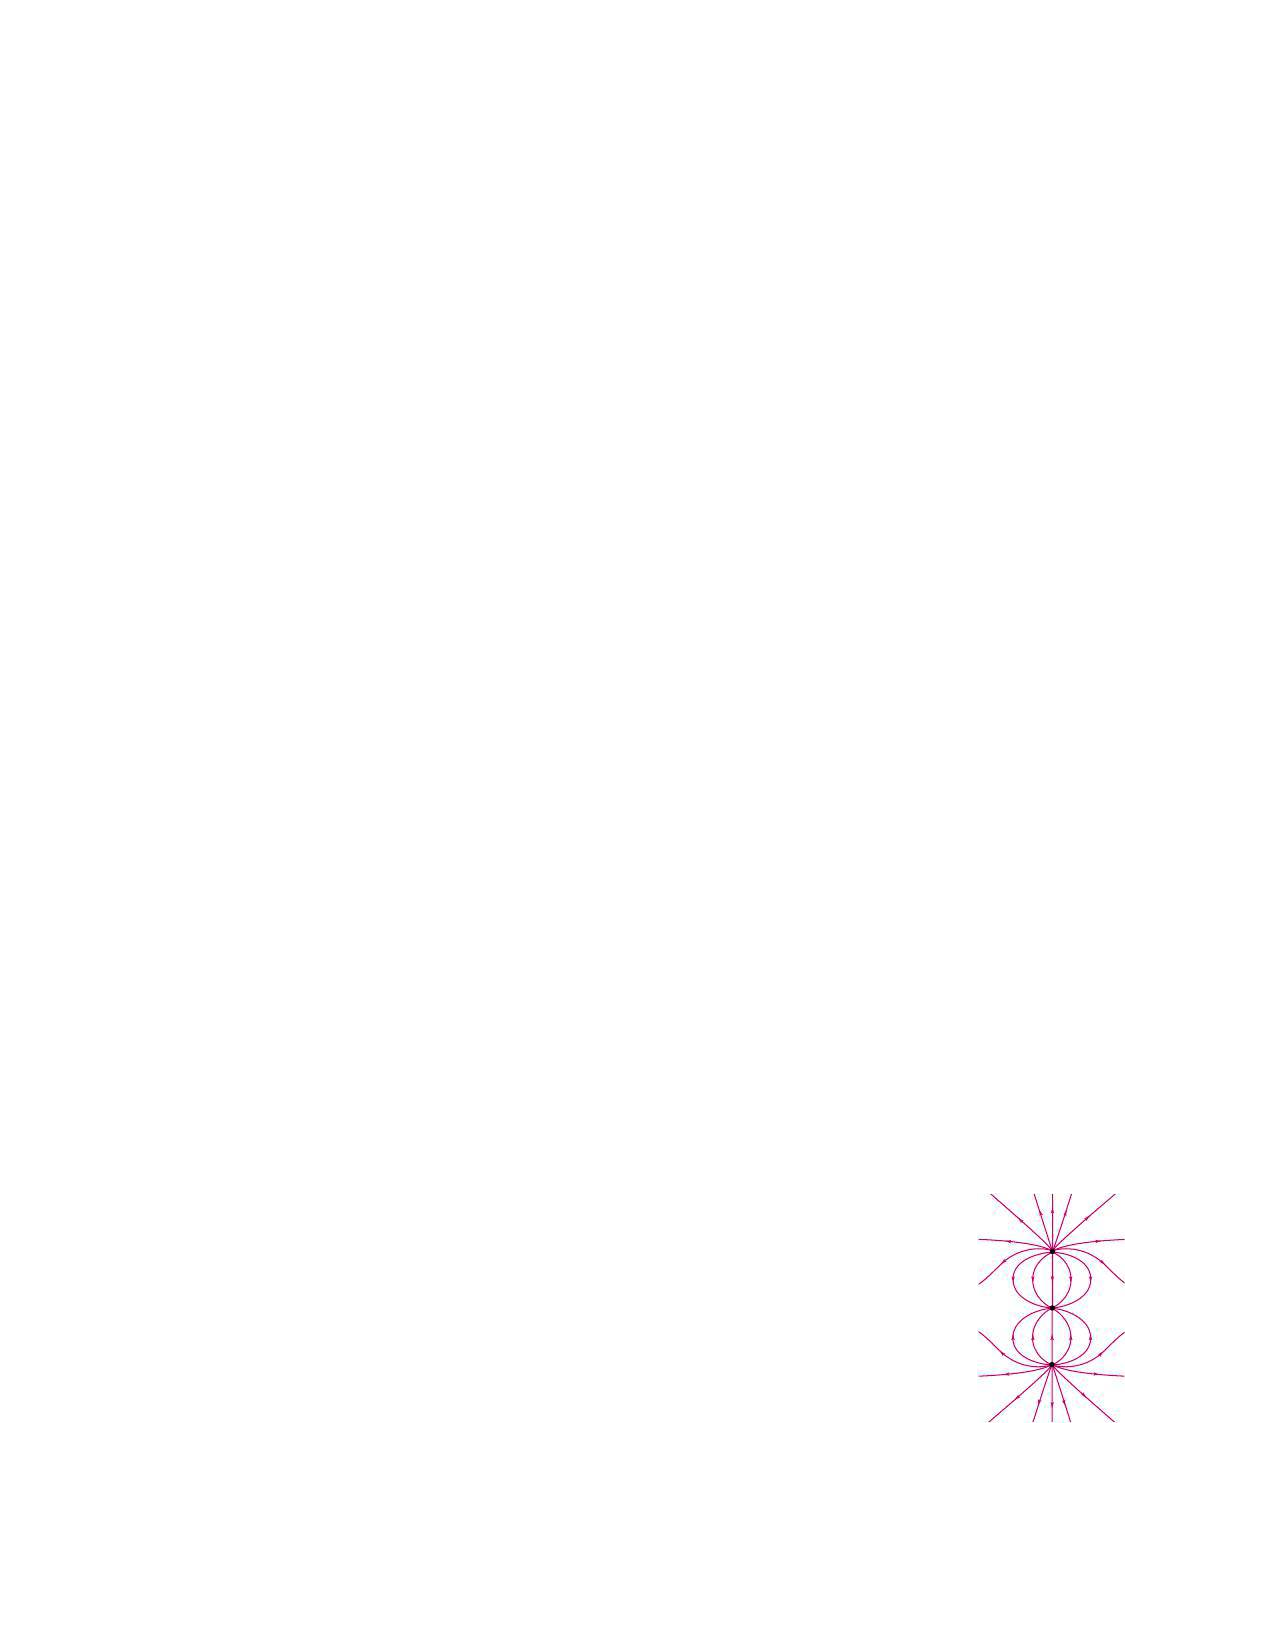
\includegraphics[scale=\imgscale]{Q21-7} & 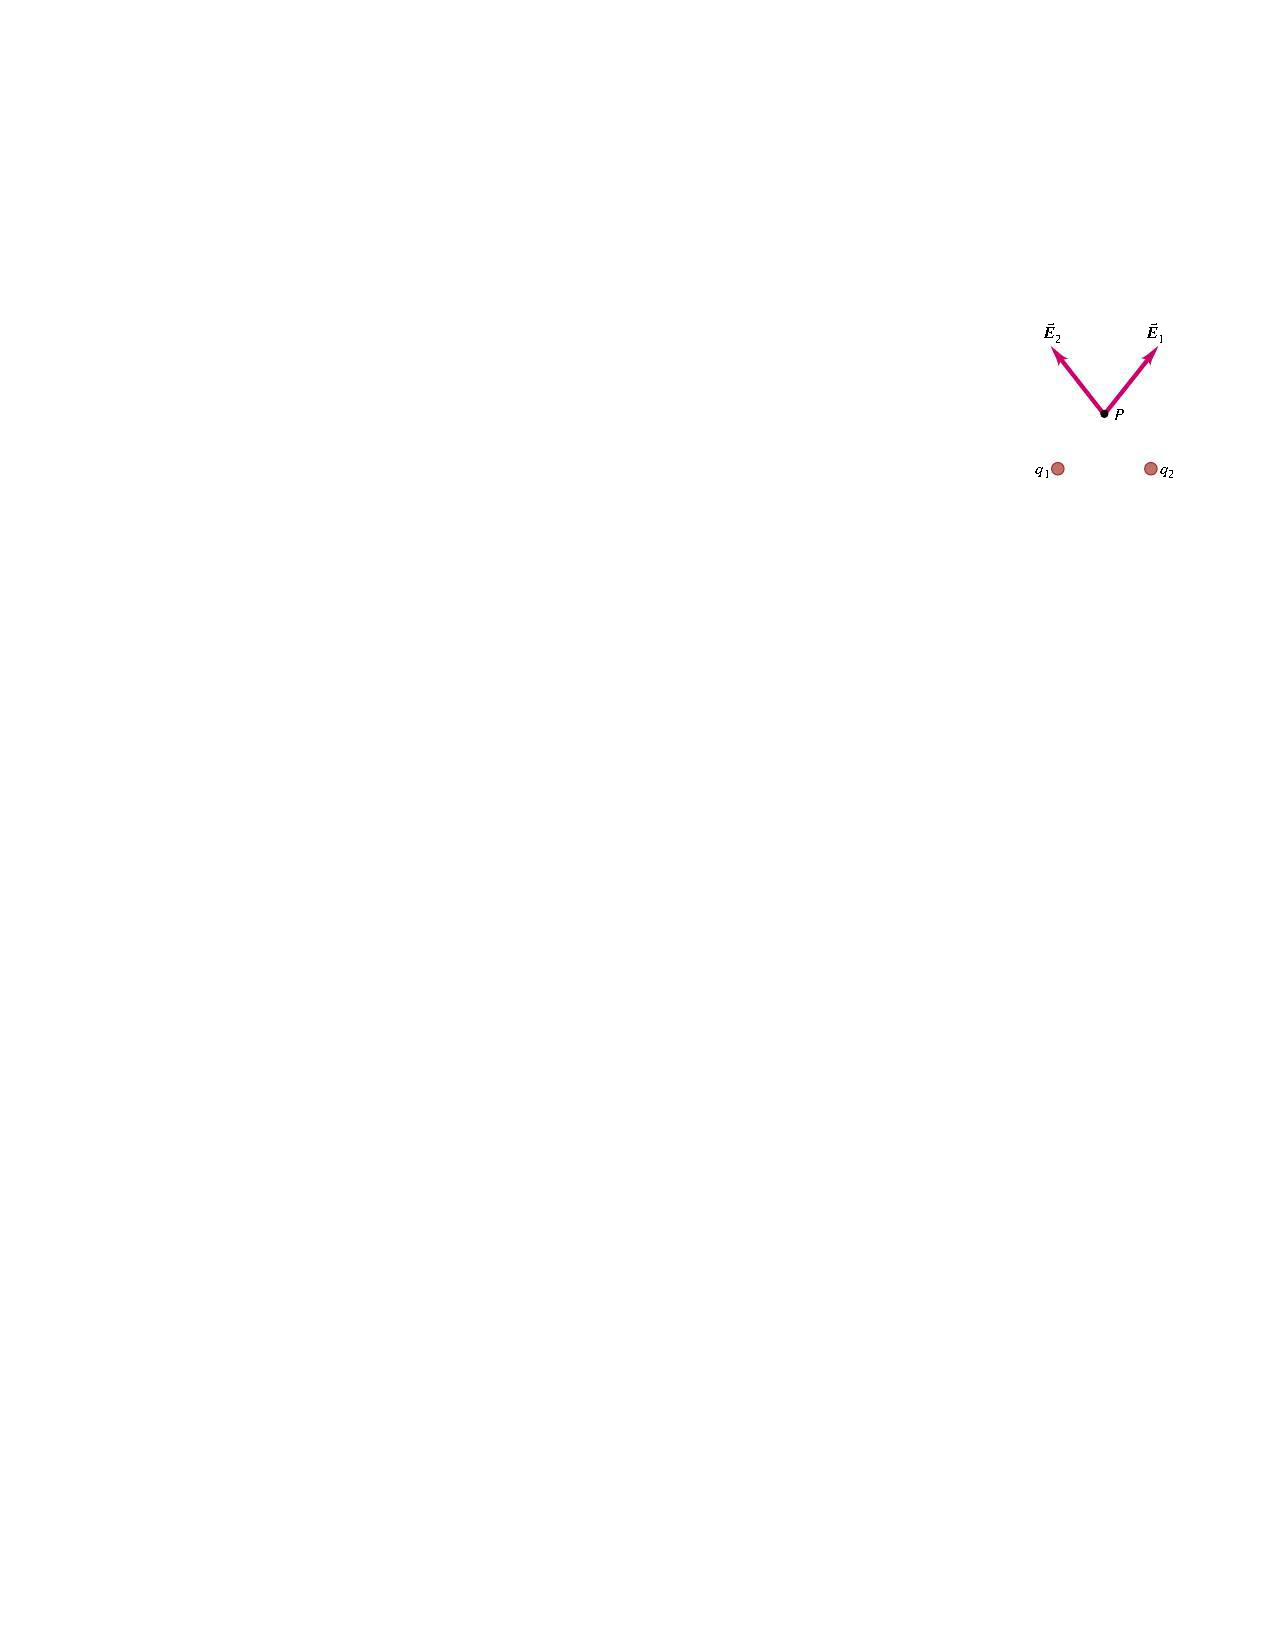
\includegraphics[scale=\imgscale]{Q21-22} & 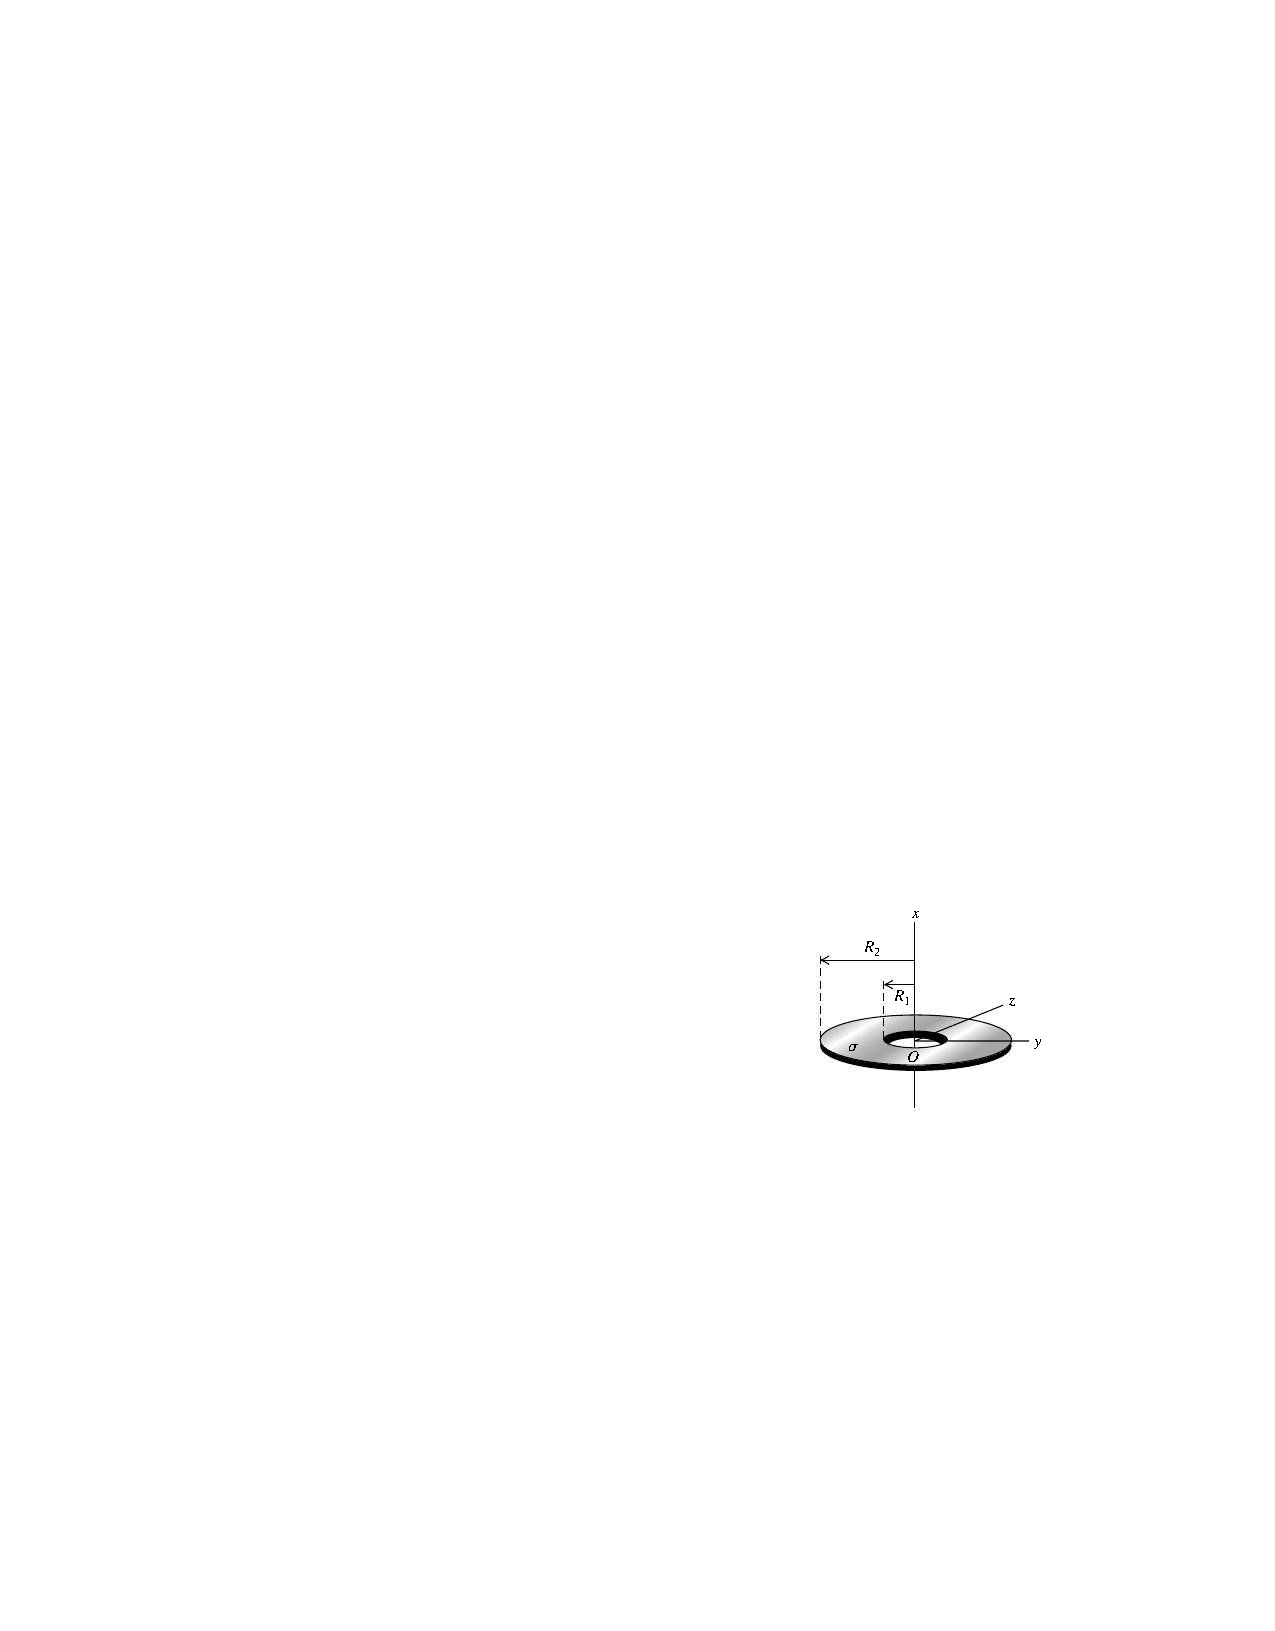
\includegraphics[scale=\imgscale]{P21-87} \\
	\textbf{Figure Q21.7} & \textbf{Figure Q21.22} & \textbf{Figure P21.87} \\
\end{tabular}
	

\bigskip\bigskip

\paragraph{Question 21.7}
\begin{problem}
	Figure Q21.7 shows some of the electric field lines due to three point charges arranged along the vertical axis.  All three charges have the same magnitude.
	
	\begin{enumerate}
		\item What are the signs of the three charges?  Explain your reasoning.
		\item At what point(s) is the magnitude of the electric field the smallest?  Explain your reasoning.  Explain how the fields produced by each individual point charge combine to give a small net field at this point or points.
	\end{enumerate}
\end{problem}

\bigskip

\paragraph{Question 21.16}
\begin{problem}
	A proton is placed in a uniform electric field and then released.  Then an electron is placed at this same point and released.  Do these particles experience the same force?  The same acceleration?  Do they move in the same direction when released?
\end{problem}

\bigskip

\paragraph{Question 21.22}
\begin{problem}
	The electric field at point $P$ due to the positive charges $q_1$ and $q_2$ are shown in Fig. Q21.22.  Does the fact that they cross each other violate the statement in Section~21.6 that electric field lines never cross?  Explain.
\end{problem}

\bigskip

\paragraph{Problem 21.69}
\begin{problem}
	A charge $+Q$ is located at the origin, and a charge $+4Q$ is at distance $d$ away on the $x$-axis.  Where should a third charge, $q$, be placed, and what should be its sign and magnitude, so that all three charges will be in equilibrium?
\end{problem}

\bigskip

\paragraph{Problem 21.87}
\begin{problem}
	A thin disk with a circular hole at its center, called an \emph{annulus}, has inner radius $R_1$ and outer radius $R_2$ (Fig. P21.87).  The disk has a uniform positive surface charge density $\sigma$ on its surface.
	\begin{enumerate}
		\item Determine the total electric charge on the annulus.
		\item The annulus lies in the $yz$-plane, with its center at the origin.  For an arbitrary point on the $x$-axis (the axis of the annulus), find the magnitude and direction of the electric field $\vec{E}$.  Consider points both above and below the annulus.
	\end{enumerate}
\end{problem}

\end{document}